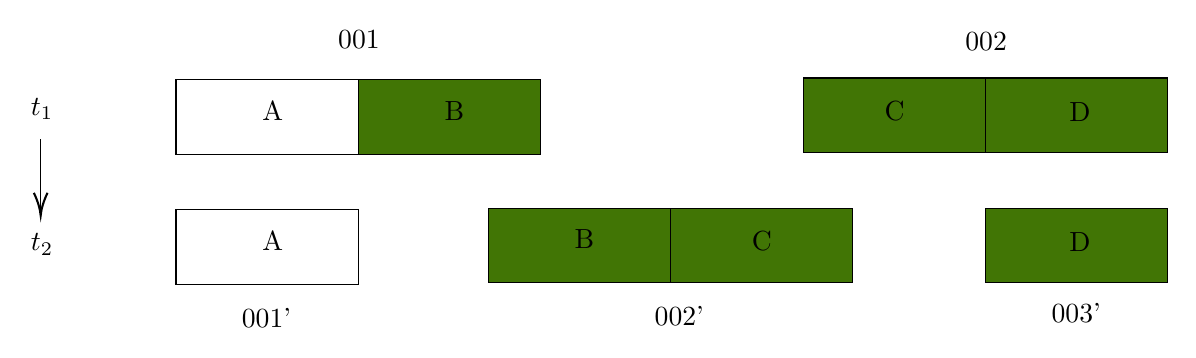
\begin{tikzpicture}[x=0.75pt,y=0.75pt,yscale=-1,xscale=1]

%Shape: Rectangle [id:dp0883975175930285] 
\draw   (133.32,62.61) -- (221.09,62.61) -- (221.09,98.42) -- (133.32,98.42) -- cycle ;
%Shape: Rectangle [id:dp1632055162352566] 
\draw  [fill={rgb, 255:red, 65; green, 117; blue, 5 }  ,fill opacity=1 ] (221.09,62.61) -- (308.85,62.61) -- (308.85,98.42) -- (221.09,98.42) -- cycle ;
%Shape: Rectangle [id:dp11080612066675233] 
\draw  [fill={rgb, 255:red, 65; green, 117; blue, 5 }  ,fill opacity=1 ] (435.48,61.71) -- (523.24,61.71) -- (523.24,97.52) -- (435.48,97.52) -- cycle ;
%Shape: Rectangle [id:dp014365723461669866] 
\draw  [fill={rgb, 255:red, 65; green, 117; blue, 5 }  ,fill opacity=1 ] (523.24,61.71) -- (611,61.71) -- (611,97.52) -- (523.24,97.52) -- cycle ;
%Shape: Rectangle [id:dp8752660840815492] 
\draw   (133.32,125.27) -- (221.09,125.27) -- (221.09,161.08) -- (133.32,161.08) -- cycle ;
%Shape: Rectangle [id:dp07344957977811539] 
\draw  [fill={rgb, 255:red, 65; green, 117; blue, 5 }  ,fill opacity=1 ] (283.77,124.38) -- (371.53,124.38) -- (371.53,160.19) -- (283.77,160.19) -- cycle ;
%Shape: Rectangle [id:dp7592509207905589] 
\draw  [fill={rgb, 255:red, 65; green, 117; blue, 5 }  ,fill opacity=1 ] (371.53,124.38) -- (459.3,124.38) -- (459.3,160.19) -- (371.53,160.19) -- cycle ;
%Shape: Rectangle [id:dp8231707743301324] 
\draw  [fill={rgb, 255:red, 65; green, 117; blue, 5 }  ,fill opacity=1 ] (523.24,124.38) -- (611,124.38) -- (611,160.19) -- (523.24,160.19) -- cycle ;
%Straight Lines [id:da043065386457907584] 
\draw    (68.13,91.25) -- (68.13,125.96) ;
\draw [shift={(68.13,127.96)}, rotate = 270] [color={rgb, 255:red, 0; green, 0; blue, 0 }  ][line width=0.75]    (10.93,-3.29) .. controls (6.95,-1.4) and (3.31,-0.3) .. (0,0) .. controls (3.31,0.3) and (6.95,1.4) .. (10.93,3.29)   ;

% Text Node
\draw (173.71,71.56) node [anchor=north west][inner sep=0.75pt]   [align=left] {A};
% Text Node
\draw (261.47,71.56) node [anchor=north west][inner sep=0.75pt]   [align=left] {B};
% Text Node
\draw (473.48,71.56) node [anchor=north west][inner sep=0.75pt]   [align=left] {C};
% Text Node
\draw (562.5,72.46) node [anchor=north west][inner sep=0.75pt]   [align=left] {D};
% Text Node
\draw (173.71,134.23) node [anchor=north west][inner sep=0.75pt]   [align=left] {A};
% Text Node
\draw (324.16,133.33) node [anchor=north west][inner sep=0.75pt]   [align=left] {B};
% Text Node
\draw (409.54,134.23) node [anchor=north west][inner sep=0.75pt]   [align=left] {C};
% Text Node
\draw (562.5,135.13) node [anchor=north west][inner sep=0.75pt]   [align=left] {D};
% Text Node
\draw (62.13,70.23) node [anchor=north west][inner sep=0.75pt]    {$t_1$};
% Text Node
\draw (62.13,135.58) node [anchor=north west][inner sep=0.75pt]    {$t_2$};
% Text Node
\draw (210.22,37.72) node [anchor=north west][inner sep=0.75pt]   [align=left] {001};
% Text Node
\draw (512.39,38.79) node [anchor=north west][inner sep=0.75pt]   [align=left] {002};
% Text Node
\draw (163.78,171.28) node [anchor=north west][inner sep=0.75pt]   [align=left] {001'};
% Text Node
\draw (362.68,170.21) node [anchor=north west][inner sep=0.75pt]   [align=left] {002'};
% Text Node
\draw (553.93,169.14) node [anchor=north west][inner sep=0.75pt]   [align=left] {003'};


\end{tikzpicture}
